\documentclass[english,,man]{apa6}
\usepackage{lmodern}
\usepackage{amssymb,amsmath}
\usepackage{ifxetex,ifluatex}
\usepackage{fixltx2e} % provides \textsubscript
\ifnum 0\ifxetex 1\fi\ifluatex 1\fi=0 % if pdftex
  \usepackage[T1]{fontenc}
  \usepackage[utf8]{inputenc}
\else % if luatex or xelatex
  \ifxetex
    \usepackage{mathspec}
  \else
    \usepackage{fontspec}
  \fi
  \defaultfontfeatures{Ligatures=TeX,Scale=MatchLowercase}
\fi
% use upquote if available, for straight quotes in verbatim environments
\IfFileExists{upquote.sty}{\usepackage{upquote}}{}
% use microtype if available
\IfFileExists{microtype.sty}{%
\usepackage{microtype}
\UseMicrotypeSet[protrusion]{basicmath} % disable protrusion for tt fonts
}{}
\usepackage{hyperref}
\hypersetup{unicode=true,
            pdftitle={Inferences With Longitudinal Data},
            pdfauthor={\ldots{}},
            pdfkeywords={\ldots{}.},
            pdfborder={0 0 0},
            breaklinks=true}
\urlstyle{same}  % don't use monospace font for urls
\ifnum 0\ifxetex 1\fi\ifluatex 1\fi=0 % if pdftex
  \usepackage[shorthands=off,main=english]{babel}
\else
  \usepackage{polyglossia}
  \setmainlanguage[]{english}
\fi
\usepackage{color}
\usepackage{fancyvrb}
\newcommand{\VerbBar}{|}
\newcommand{\VERB}{\Verb[commandchars=\\\{\}]}
\DefineVerbatimEnvironment{Highlighting}{Verbatim}{commandchars=\\\{\}}
% Add ',fontsize=\small' for more characters per line
\usepackage{framed}
\definecolor{shadecolor}{RGB}{248,248,248}
\newenvironment{Shaded}{\begin{snugshade}}{\end{snugshade}}
\newcommand{\AlertTok}[1]{\textcolor[rgb]{0.94,0.16,0.16}{#1}}
\newcommand{\AnnotationTok}[1]{\textcolor[rgb]{0.56,0.35,0.01}{\textbf{\textit{#1}}}}
\newcommand{\AttributeTok}[1]{\textcolor[rgb]{0.77,0.63,0.00}{#1}}
\newcommand{\BaseNTok}[1]{\textcolor[rgb]{0.00,0.00,0.81}{#1}}
\newcommand{\BuiltInTok}[1]{#1}
\newcommand{\CharTok}[1]{\textcolor[rgb]{0.31,0.60,0.02}{#1}}
\newcommand{\CommentTok}[1]{\textcolor[rgb]{0.56,0.35,0.01}{\textit{#1}}}
\newcommand{\CommentVarTok}[1]{\textcolor[rgb]{0.56,0.35,0.01}{\textbf{\textit{#1}}}}
\newcommand{\ConstantTok}[1]{\textcolor[rgb]{0.00,0.00,0.00}{#1}}
\newcommand{\ControlFlowTok}[1]{\textcolor[rgb]{0.13,0.29,0.53}{\textbf{#1}}}
\newcommand{\DataTypeTok}[1]{\textcolor[rgb]{0.13,0.29,0.53}{#1}}
\newcommand{\DecValTok}[1]{\textcolor[rgb]{0.00,0.00,0.81}{#1}}
\newcommand{\DocumentationTok}[1]{\textcolor[rgb]{0.56,0.35,0.01}{\textbf{\textit{#1}}}}
\newcommand{\ErrorTok}[1]{\textcolor[rgb]{0.64,0.00,0.00}{\textbf{#1}}}
\newcommand{\ExtensionTok}[1]{#1}
\newcommand{\FloatTok}[1]{\textcolor[rgb]{0.00,0.00,0.81}{#1}}
\newcommand{\FunctionTok}[1]{\textcolor[rgb]{0.00,0.00,0.00}{#1}}
\newcommand{\ImportTok}[1]{#1}
\newcommand{\InformationTok}[1]{\textcolor[rgb]{0.56,0.35,0.01}{\textbf{\textit{#1}}}}
\newcommand{\KeywordTok}[1]{\textcolor[rgb]{0.13,0.29,0.53}{\textbf{#1}}}
\newcommand{\NormalTok}[1]{#1}
\newcommand{\OperatorTok}[1]{\textcolor[rgb]{0.81,0.36,0.00}{\textbf{#1}}}
\newcommand{\OtherTok}[1]{\textcolor[rgb]{0.56,0.35,0.01}{#1}}
\newcommand{\PreprocessorTok}[1]{\textcolor[rgb]{0.56,0.35,0.01}{\textit{#1}}}
\newcommand{\RegionMarkerTok}[1]{#1}
\newcommand{\SpecialCharTok}[1]{\textcolor[rgb]{0.00,0.00,0.00}{#1}}
\newcommand{\SpecialStringTok}[1]{\textcolor[rgb]{0.31,0.60,0.02}{#1}}
\newcommand{\StringTok}[1]{\textcolor[rgb]{0.31,0.60,0.02}{#1}}
\newcommand{\VariableTok}[1]{\textcolor[rgb]{0.00,0.00,0.00}{#1}}
\newcommand{\VerbatimStringTok}[1]{\textcolor[rgb]{0.31,0.60,0.02}{#1}}
\newcommand{\WarningTok}[1]{\textcolor[rgb]{0.56,0.35,0.01}{\textbf{\textit{#1}}}}
\usepackage{graphicx,grffile}
\makeatletter
\def\maxwidth{\ifdim\Gin@nat@width>\linewidth\linewidth\else\Gin@nat@width\fi}
\def\maxheight{\ifdim\Gin@nat@height>\textheight\textheight\else\Gin@nat@height\fi}
\makeatother
% Scale images if necessary, so that they will not overflow the page
% margins by default, and it is still possible to overwrite the defaults
% using explicit options in \includegraphics[width, height, ...]{}
\setkeys{Gin}{width=\maxwidth,height=\maxheight,keepaspectratio}
\IfFileExists{parskip.sty}{%
\usepackage{parskip}
}{% else
\setlength{\parindent}{0pt}
\setlength{\parskip}{6pt plus 2pt minus 1pt}
}
\setlength{\emergencystretch}{3em}  % prevent overfull lines
\providecommand{\tightlist}{%
  \setlength{\itemsep}{0pt}\setlength{\parskip}{0pt}}
\setcounter{secnumdepth}{0}
% Redefines (sub)paragraphs to behave more like sections
\ifx\paragraph\undefined\else
\let\oldparagraph\paragraph
\renewcommand{\paragraph}[1]{\oldparagraph{#1}\mbox{}}
\fi
\ifx\subparagraph\undefined\else
\let\oldsubparagraph\subparagraph
\renewcommand{\subparagraph}[1]{\oldsubparagraph{#1}\mbox{}}
\fi

%%% Use protect on footnotes to avoid problems with footnotes in titles
\let\rmarkdownfootnote\footnote%
\def\footnote{\protect\rmarkdownfootnote}


  \title{Inferences With Longitudinal Data}
    \author{\ldots{}\textsuperscript{1}}
    \date{}
  
\shorttitle{LONGITUDINAL INFERENCES}
\affiliation{
\vspace{0.5cm}
\textsuperscript{1} ...}
\keywords{....\newline\indent Word count: 95}
\usepackage{csquotes}
\usepackage{upgreek}
\captionsetup{font=singlespacing,justification=justified}

\usepackage{longtable}
\usepackage{lscape}
\usepackage{multirow}
\usepackage{tabularx}
\usepackage[flushleft]{threeparttable}
\usepackage{threeparttablex}

\newenvironment{lltable}{\begin{landscape}\begin{center}\begin{ThreePartTable}}{\end{ThreePartTable}\end{center}\end{landscape}}

\makeatletter
\newcommand\LastLTentrywidth{1em}
\newlength\longtablewidth
\setlength{\longtablewidth}{1in}
\newcommand{\getlongtablewidth}{\begingroup \ifcsname LT@\roman{LT@tables}\endcsname \global\longtablewidth=0pt \renewcommand{\LT@entry}[2]{\global\advance\longtablewidth by ##2\relax\gdef\LastLTentrywidth{##2}}\@nameuse{LT@\roman{LT@tables}} \fi \endgroup}


\DeclareDelayedFloatFlavor{ThreePartTable}{table}
\DeclareDelayedFloatFlavor{lltable}{table}
\DeclareDelayedFloatFlavor*{longtable}{table}
\makeatletter
\renewcommand{\efloat@iwrite}[1]{\immediate\expandafter\protected@write\csname efloat@post#1\endcsname{}}
\makeatother
\usepackage{lineno}

\linenumbers

\authornote{\ldots{}.

Correspondence concerning this article should be addressed to \ldots{},
\ldots{}. E-mail: \ldots{}}

\abstract{
Begin here\ldots{}


}

\usepackage{amsthm}
\newtheorem{theorem}{Theorem}[section]
\newtheorem{lemma}{Lemma}[section]
\theoremstyle{definition}
\newtheorem{definition}{Definition}[section]
\newtheorem{corollary}{Corollary}[section]
\newtheorem{proposition}{Proposition}[section]
\theoremstyle{definition}
\newtheorem{example}{Example}[section]
\theoremstyle{definition}
\newtheorem{exercise}{Exercise}[section]
\theoremstyle{remark}
\newtheorem*{remark}{Remark}
\newtheorem*{solution}{Solution}
\begin{document}
\maketitle

Organizational phenomena unfold over time. They are processes that
develop, change, and evolve (Pitariu \& Ployhart, 2010) that create a
sequence of events within a person's stream of experience (Beal, 2015).
Moreover, organizations are systems with many connected parts, and
systems are inherently dynamic. Studying these systems and processes,
therefore, requires paying attention not to static snapshots of behavior
(Ilgen \& Hulin, 2000), but to variables and relationships as they move
through time; doing so puts us in a better position to capture the
sequence, understand it, and can lead to new and interesting insights
(Kozlowski \& Bell, 2003).

This sentiment is reflected in our empirical literature, where repeated
assessments are now common. For instance, Jones et al. (2016) observed
the work attitudes of pregnant women in their second trimester every
week until they gave birth. Meier and Spector (2013) examined
counterproductive work behavior over five waves. Hardy, Day, and Steele
(2018) investigated self-regulation over 20 lab trials. Finally,
Johnson, Lanaj, and Barnes (2014) observed justice behavior and resource
depletion across 10 consecutive workdays.

Armed with repeated observations, there are then different research
questions that we can explore. Jones et al. (2016) ask about trend: they
want to determine if the trajectories among certain variables increase
or decrease over time. Johnson et al. (2014) about change: they are
interested in how changes in one variable relate to changes in another
across time. Hardy et al. (2018) inquire about dynamic relationships,
where prior values on one variable predict subsequent values on another,
and this second variable then goes back to predict the first at a later
point in time. Finally, Meier and Spector (2013) examine how effect
sizes change when they vary the time lag between their independent and
dependent variable.

Researchers then evoke statistical models that are determined by their
research questions. Meier and Spector (2013) present a sequence of path
models that test increasingly longer time lags. Hardy et al. (2018) and
Jones et al. (2016) employ bivariate cross-lagged latent growth curves,
an approach similar to the latent change model used by Ritter, Matthews,
Ford, and Henderson (2016). We also find complex hierarchical linear
models in many event-sampling studies (e.g., Koopman, Lanaj, \& Scott,
2016; Rosen, Koopman, Gabriel, \& Johnson, 2016).

The spine of an investigation, finally, is to interpret the model and
make an inference regarding the original question. Jones et al. (2016)
infer negative slopes for concealing behaviors and positive slopes for
revealing behaviors. Johnson et al. (2014) state that justice behaviors
fluctuate day to day and predict changes in depletion. Hardy et al.
(2018) find support for dynamic relationships between self-efficacy,
metacognition, and exploratory behaviors. Finally, Meier and Spector
(2013) suggest that the effects of work stressors on counterproductive
work behaviors are not substantially different across different time
lags.

None of these inferences perfectly discovers the data generating
mechanism. Rather, each asks an interesting and important question about
how DVs relate to IVs. Only with lots of asking about lots of different
patterns of relationships across the variables could we piece together
one (of many) possible representation(s) of the data generating process
-- hopefully having a good theory to guide the way.

We want to link inferences to models in this paper so that researchers
know which of the many models they can use when they are interested in
one of the many possible inferences in a longitudinal investigation. As
should be clear to anyone reading our literature, there is great
excitement for the utility of longitudinal studies; they can pose
interesting questions and discover patterns that would otherwise be
impossible to capture in a static investigation. We bring attention to
the span of questions available so that researchers can fully appreciate
and take advantage of their data. Although the inferences concern
trajectories or relationships over time, their small differences have
large implications for what we take away from them -- what we ultimately
conclude. Moreoever, there are many inferences, many models, and
different models can be used to understand or explore the same
inference. In this paper, we provide readers with potential models for
each inference so that they can be sure that the model they evoke is
appropriate for the research question that they are interested in. In
summary, this paper exposes researchers to the span of inferences they
may investigate when they collect longitudinal data, links those
inferences to models, and parses some of the modeling literature that
may be difficult to consume for researchers with only graduate level
training in statistics.

Below, we do these things.

\hypertarget{longitudinal-definitions}{%
\section{Longitudinal Definitions}\label{longitudinal-definitions}}

This paper is exclusively devoted to the inferences we make with
repeated observations, so we begin by identifying a few labels and
definitions. Authors typically identify a \enquote{longitudinal} study
by making a contrast with respect to either a) research designs or b)
data structures. Longitudinal \emph{research} is different from
cross-sectional research because longitudinal designs entail three or
more repeated observations (Ployhart \& Vandenberg, 2010). We therefore
emphasize differences on the number of observations when we distinguish
longitudinal from other types of research. Longitudinal \emph{data} are
repeated observations on several units (i.e., \(N\) or \(i\)
\textgreater{} 1), whereas panel data are observations of one unit over
time -- a distinction that focuses on the amount of people in our study
(given repeated measures). Most organizational studies collect data on
more than one unit, therefore our discussion below focuses on
longitudinal research with longitudinal data, or designs with \(N\)
\textgreater{} 1, \(t\) \textgreater{}= 3, and the same construct(s)
measured on each \(i\) at each \(t\).

\hypertarget{framework}{%
\subsection{Framework}\label{framework}}

Level. Trend. Dynamics. These are umbrella research foci, each has its
own sub-inferences and models. Each section will have several inferences
but they all gather into two basic notions: 1) trying to understand the
thing itself and variability about the thing itself across units, and 2)
correlates or predictors of the thing.

Each section will also point to models. But there is nuance. The models
have different names, some require stationary, some don't. You need to
appreciate that and make sure you are attending to all of its nuance.
All we are doing here is pointing you in the direction.

\hypertarget{level}{%
\section{Level}\label{level}}

Is employee emotional exhaustion, on average, high across the study? Is
trainee skill low at the beginning of a training session? What value are
newcomer perceptions of unit climate at the end of a two-week
socialization process? These are questions about level, or the specific
value of a variable.

Levels either describe the variable at one moment or averaged across a
span of time. That is, if we put a variable on the \(y\) axis and plot
its values against time on the \(x\) axis, we can explore the value that
it takes at time \(t\), or the value that it takes on average across any
span of \(t\).

Figure \ref{level} demonstrates this idea graphically. A variable is
plotted across time, and the color labels indicate levels -- the red and
green describe the variable at a specific moment while the purple,
average level, describes it across a window.

\begin{center}

------------

Insert Figure \ref{level} about here

------------

\end{center}

\noindent Our first level inference, therefore, concerns the value of a
variable at a specific time or averaged across a window of time.

\hypertarget{inference-1-what-is-the-level-of-x-at-time-t-or-across-a-span-of-t}{%
\paragraph{\texorpdfstring{Inference 1: What is the level of \(x\) at
time \(t\), or across a span of
\(t\)?}{Inference 1: What is the level of x at time t, or across a span of t?}}\label{inference-1-what-is-the-level-of-x-at-time-t-or-across-a-span-of-t}}

When we retain one variable but add multiple units -- people or
organizations, for example -- then we can look at the variability in
level. Does everyone have high affect across time? Is there variability
in the level of skill among trainees at the beginning of a training
session?

We demonstrate this idea in figure \ref{level_var}, where each unit
(person) has a similar trajectory but different levels at the last time
point.

\begin{center}

------------

Insert Figure \ref{level_var} about here

------------

\end{center}

\noindent The second level inference, therefore, is about level
variability across units.

\hypertarget{inference-2-across-a-span-of-t-or-at-a-specific-t-there-is-variability-in-the-level-of-x.}{%
\paragraph{\texorpdfstring{Inference 2: Across a span of \(t\) or at a
specific \(t\) there is variability in the level of
\(x\).}{Inference 2: Across a span of t or at a specific t there is variability in the level of x.}}\label{inference-2-across-a-span-of-t-or-at-a-specific-t-there-is-variability-in-the-level-of-x.}}

Inferences one and two concern a single variable, but they can of course
be iterated across any or all observed variables in the study. For
example, we might discover that affect and performance have high average
levels across time, but that affect has greater level variability. Or we
might learn that affect has a low initial level whereas performance is
initially high. What we are doing here is making descriptive comparisons
between the level of one variable and the level of another. We can also
produce a quantitative statement about the extent to which levels are
related.

Correlating levels provides us with that quantitative statement. A large
positive correlation between the initial levels of affect and
performance would mean that people with greater initial levels of affect
also tend to have greater intial performance, and people with lower
initial affect also tend to have lower initial performance.

Figure \ref{level_correlate} (no figure yet) demonstrates this
graphically. Paragraph about the graph.

\hypertarget{inference-3-there-is-a-correlation-between-the-level-of-x-and-y-at-t.}{%
\paragraph{\texorpdfstring{Inference 3: There is a correlation between
the level of \(x\) and \(y\) at
\(t\).}{Inference 3: There is a correlation between the level of x and y at t.}}\label{inference-3-there-is-a-correlation-between-the-level-of-x-and-y-at-t.}}

The final level inference is horizontal. Rather than correlating values
from a single moment or a single averaged moment, we correlate values
across time. For example, we might ask if affect is related to
performance across time; i.e., when affect is high is performance also
high, and when affect is low is performance also low? This inference
sounds similar to the one just presented, but their difference is
important. With inference three we ask about affect and performance at
\(t\) or at an averaged window of \(t\) -- we examine how averaged
values across time relate to averaged values across time, for example.
Here, we retain all of the information and examine the relationship
between affect and performance across all \(t\).

Figure \ref{level_relation} shows this inference graphically. The top
panel plots affect and performance trajectories across time. The colored
squares represent levels at different points in time. The green squares
highlight low values of both variables, the blue high values, and the
red middle values. The bottom panel shows how those respective values
map onto a graph that describes the relationship between affect and
performance across time. Notice that there appears to be a positive
relationship in the scatterplot, which tells us that when affect is high
performance also tends to be high, and vice versa.

\begin{center}

------------

Insert Figure \ref{level_relation} about here

------------

\end{center}

\hypertarget{inference-4-there-is-a-relationship-between-x-and-y-across-time.}{%
\paragraph{\texorpdfstring{Inference 4: There is a relationship between
\(x\) and \(y\) across
time.}{Inference 4: There is a relationship between x and y across time.}}\label{inference-4-there-is-a-relationship-between-x-and-y-across-time.}}

\hypertarget{level-inference-table}{%
\subsection{Level Inference Table}\label{level-inference-table}}

The inference table below provides examples of each level inference.
Inference one is about level itself -- a single value that describes the
variable at one time or averaged across time. Inference two is about
variability across units in level. Inference three takes the level in
one variable and asks whether it tends to co-occur with the level in
another. Think of inference three as creating a latent level variable at
a single moment and asking how it relates to another latent variable
from a single momoment. Inference four, finally, is about the
relationship between raw values across time.

\begin{tabular}{>{\raggedright\arraybackslash}p{5em}>{\raggedright\arraybackslash}p{30em}}
\toprule
Inference & Examples\\
\midrule
1 & Burnout is high at the last time point.\newline Performance is low, on average, across time.\\
\hline
2 & Average affect across time differs across people (units).\newline There is variability in the initial level of turnover across organizations.\\
\hline
3 & People with greater initial health status also have greater initial happiness.\newline People with high performance on average across time have lower anxiety on average across time.\\
\hline
4 & Affect relates to performance across time.\newline Helping behaviors predict depletion across time.\\
\bottomrule
\end{tabular}

\hypertarget{models}{%
\subsection{Models}\label{models}}

Level is called intercept in the statistical modeling literature.
Typically the mean estimate tells you about the level, and the variance
estimate tells you about the variability across units. Intercept only
models in HLM or SEM. Time-varying or invariant covariates analyses.
Point to references.

\begin{figure}
\centering
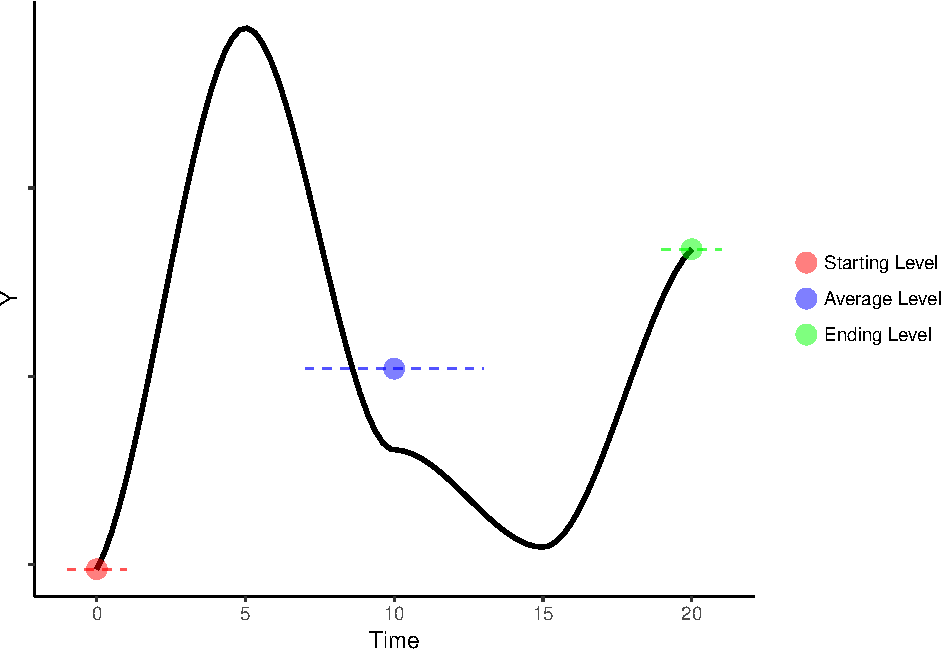
\includegraphics{figures/unnamed-chunk-8-1.pdf}
\caption{\label{fig:unnamed-chunk-8}Level examples\label{level}}
\end{figure}

\begin{figure}
\centering
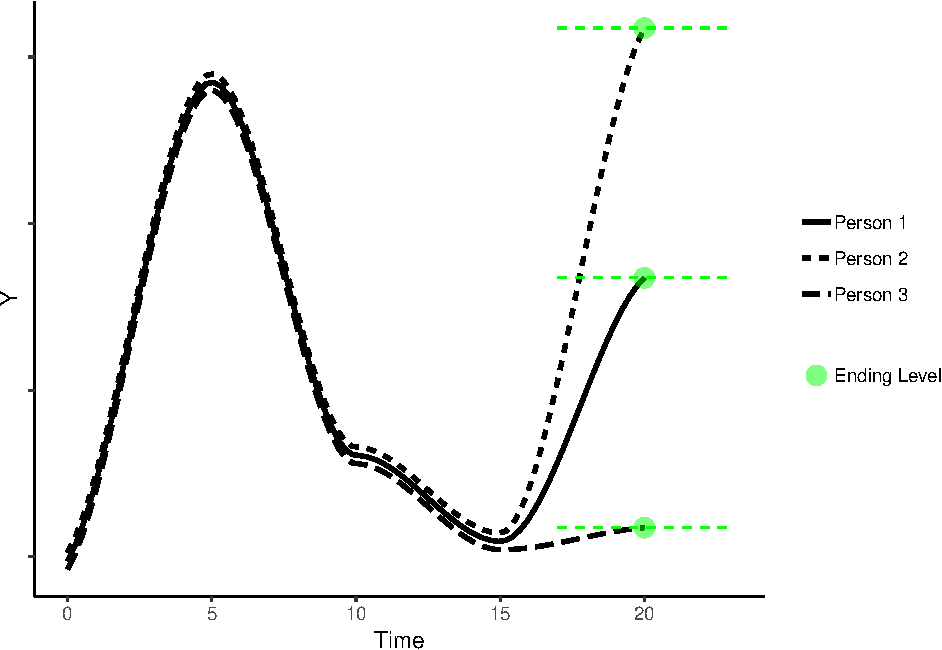
\includegraphics{figures/unnamed-chunk-9-1.pdf}
\caption{\label{fig:unnamed-chunk-9}Trajectories with variability in ending
level across units\label{level_var}}
\end{figure}

\begin{figure}
\centering
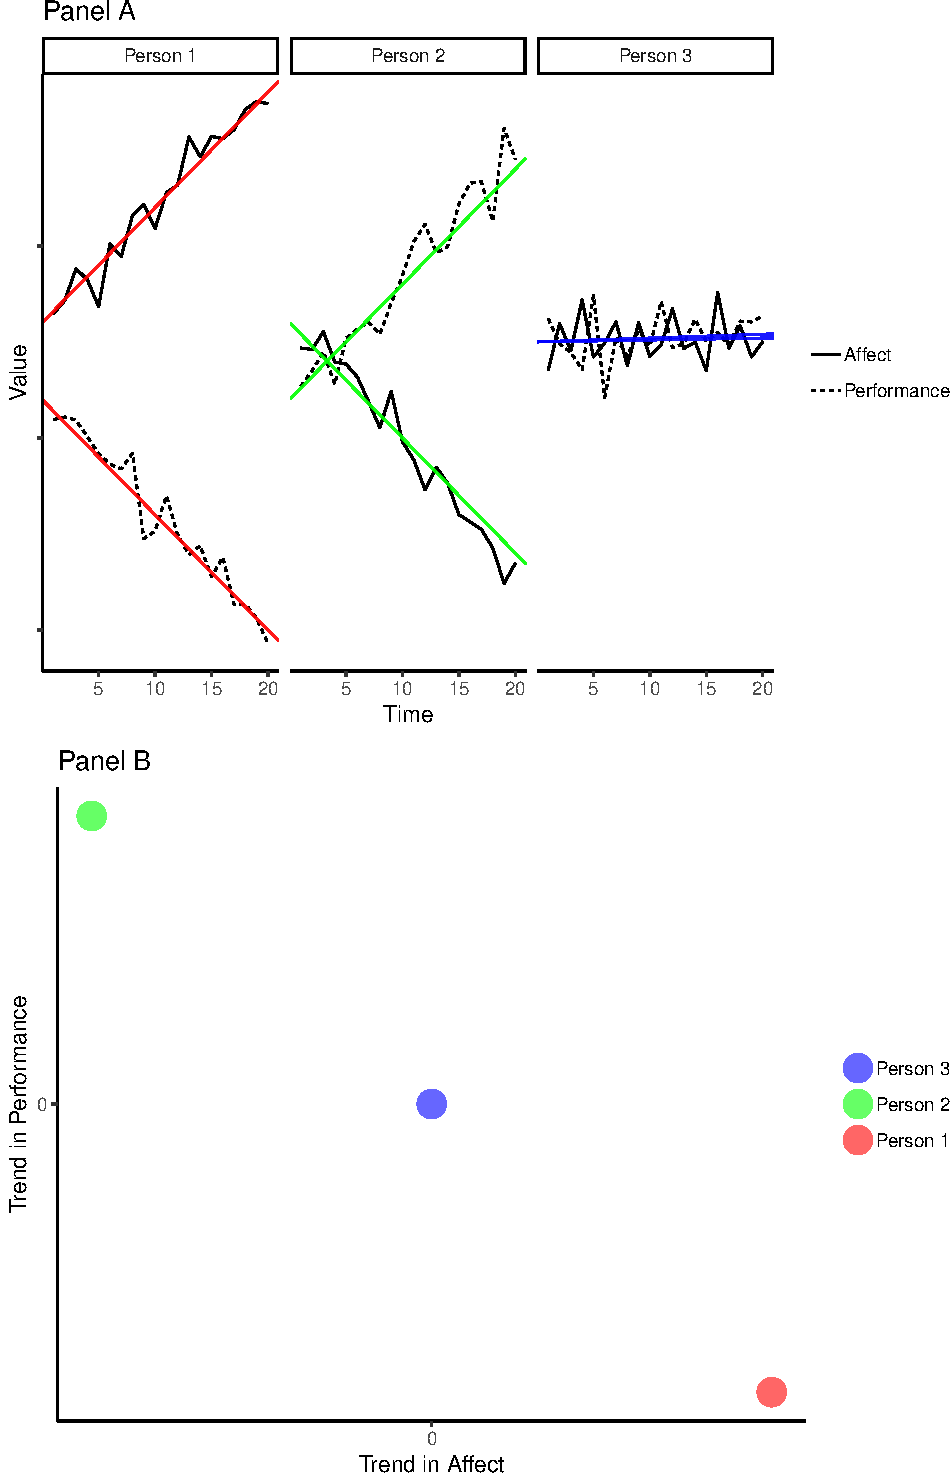
\includegraphics{figures/unnamed-chunk-10-1.pdf}
\caption{\label{fig:unnamed-chunk-10}Relating affect to performance
levels\label{level_relation}}
\end{figure}

\hypertarget{trend}{%
\section{Trend}\label{trend}}

Does affect go up or down across time, or is it relatively stable? Does
trainee skill increase over the training session? These are questions
about trend, and these first two are specifically about linear trend. It
is also possible to explore how variables bend or curve across time. Do
newcomer perceptions of climate increase and then plateau over time?
Does the response time of a medical team decrease with each successive
case but then remain stable once the team can no longer improve their
coordination? These latter questions concern curvilinear trajectories.

Trend has to do with the global shape of the trajectory across time. If
we put a variable on the \(y\)-axis and plot its values against time on
the \(x\)-axis, do the values tend to go up or down over time? It can be
thought of as the coarse-grained direction of a trajectory.

Figure \ref{trend} demonstrates trend, where the red line shows
positive, increasing trend, the blue line shows negative, decreasing
trend, and the green line shows a curvilinear trajectory (ADD GREEN
LINE). Keep in mind that curvilinear and linear trajectories are both
\emph{linear in parameters} and should not be confused with non-linear
systems.

\begin{center}

------------

Insert Figure \ref{trend} about here

------------

\end{center}

Our first trend inference, therefore, concerns the shape of the
trajectory.

\hypertarget{inference-1-there-is-positivenegativecurvilinear-trend-in-a-variable-across-time.}{%
\paragraph{Inference 1: There is positive/negative/curvilinear trend in
a variable across
time.}\label{inference-1-there-is-positivenegativecurvilinear-trend-in-a-variable-across-time.}}

As with the level inferences, when we add more units we can examine
trend variability. Do all trainees develop greater skill across time? Is
there variability in the trend of helping behaviors, or
counterproductive work behaviors over time?

Figure \ref{trend_var} shows differences in trend variability. In the
first panel all units (people) show the same positive trend, whereas
everyone in the second panel shows different trend: person one's data
appear to increase over time, person two's data remain flat, and person
three's data decrease over time. With greater variability there is less
consistency in trend across units.

\begin{center}

------------

Insert Figure \ref{trend_var} about here

------------

\end{center}

\hypertarget{inference-2-there-is-variability-in-the-trend-of-a-variable-across-time-trend-differs-across-units.}{%
\paragraph{Inference 2: There is variability in the trend of a variable
across time; trend differs across
units.}\label{inference-2-there-is-variability-in-the-trend-of-a-variable-across-time-trend-differs-across-units.}}

Inferences one and two are about one variable, but they can also be
iterated across all observed variables. For example, we might discover
that affect and performance trends both decrease, but there is greater
variability across units in the affect trend. Or we might learn that
affect has a negative trend while performance has a positive trend.

Correlating these trends is the next inference. Just like before,
correlating indicates co-occuring patterns, but this time we are focused
on trends rather than levels. A large positive correlation between
affect and performance trends indicates that people with a positive
affect trend (usually) have a positive performance trend and people with
a negative affect trend (usually) have a negative performance trend.

Figure \ref{trend_correlation} shows the inuition behind the inference
with a set of graphs. On the top panel, affect and performance are
plotted across time for three individuals. For individual one, affect
goes up while performance goes down, this pattern is reversed for person
two, and person three reports fluctuating affect and performance but
with no trend. The bottom panel then maps those pairings onto a figure
that shows the relationship between the affect and performance trend.
For example, person one has a positive affect trend and a negative
performance trend, so their point on the bottom panel goes on the bottom
right, whereas person two has the opposite pattern and therefore is
placed on the top left (where performance trend is positive and affect
trend is negative). Producing this bottom scatter plot tells us that the
relationship between affect and performance trend is negative. That is,
people with a positive affect trend usually have a negative performance
trend.

\begin{center}

------------

Insert Figure \ref{trend_correlation} about here

------------

\end{center}

\hypertarget{inference-3-there-are-correlated-trends.-there-is-a-relationship-between-two-trends.}{%
\paragraph{Inference 3: There are correlated trends. There is a
relationship between two
trends.}\label{inference-3-there-are-correlated-trends.-there-is-a-relationship-between-two-trends.}}

The final trend inference is about identifying covariates or predictors
of trend. Do helping behaviors predict the trend in depletion? Does the
trend in unit climate covary with perceptions of leader quality?

Notice the difference between this inference and inference three.
Inference three asks how one trend is related to another, whereas this
inference asks how raw values relate to or predict the trend in a
different variable. \textbf{Note: How is this possible? Slope is a
single value, like 0.5, whereas there are as many raw values as there
are time points. So X is trying to predict Y, but X has 10 values and Y
has 1 value.}

Figure \ref{trend_relation} (no figure yet). Paragraph about graph. Not
sure what this would entail.

\hypertarget{inference-4-there-are-correlatespredictors-of-trend.}{%
\paragraph{Inference 4: There are correlates/predictors of
trend.}\label{inference-4-there-are-correlatespredictors-of-trend.}}

\hypertarget{trend-inference-table}{%
\subsection{Trend Inference Table}\label{trend-inference-table}}

The inference table below provides examples of each trend inference.
Inference one is about the general direction or shape of a trajectory
across time. Inference two is about variability in that shape across
units. Inference three takes the trend in one variable and asks whether
it tends to co-occur with trend in another. Inference four, finally, is
about the relationship between trend in one variable and the raw values
of one or more predictors.

\begin{tabular}{>{\raggedright\arraybackslash}p{5em}>{\raggedright\arraybackslash}p{30em}}
\toprule
Inference & Examples\\
\midrule
1 & Burnout decreases over time.\newline Performance increases over time.\\
\hline
2 & Affect trends differ across people (units).\newline There is variability in turnover trends across organizations.\\
\hline
3 & People with positive health status trends have positive happiness trends.\newline People with positive performance trends have negative anxiety trends.\\
\hline
4 & Affect relates to the performance trend across time.\newline Helping behaviors predict depletion trends.\\
\bottomrule
\end{tabular}

\hypertarget{a-note-on-phrasing.-correlating-trends-people-with-a-negative-affect-trend-have-a-positive-performance-trend.-this-description-is-way-different-than-when-peoples-affect-decreases-their-performance-goes-up-and-when-their-affect-increases-their-performance-goes-down.-this-second-statement-is-about-fluctuations-not-about-global-trends.-correlating-trends-only-tells-you-about-the-former-kind-of-statement.}{%
\subsubsection{\texorpdfstring{A note on phrasing. Correlating trends:
\enquote{people with a negative affect trend have a positive performance
trend.} This description IS WAY DIFFERENT THAN: when people's affect
decreases their performance goes up; and when their affect increases
their performance goes down. This second statement is about
fluctuations, not about global trends. Correlating trends only tells you
about the former kind of
statement.}{A note on phrasing. Correlating trends: ``people with a negative affect trend have a positive performance trend.'' This description IS WAY DIFFERENT THAN: when people's affect decreases their performance goes up; and when their affect increases their performance goes down. This second statement is about fluctuations, not about global trends. Correlating trends only tells you about the former kind of statement.}}\label{a-note-on-phrasing.-correlating-trends-people-with-a-negative-affect-trend-have-a-positive-performance-trend.-this-description-is-way-different-than-when-peoples-affect-decreases-their-performance-goes-up-and-when-their-affect-increases-their-performance-goes-down.-this-second-statement-is-about-fluctuations-not-about-global-trends.-correlating-trends-only-tells-you-about-the-former-kind-of-statement.}}

\begin{figure}
\centering
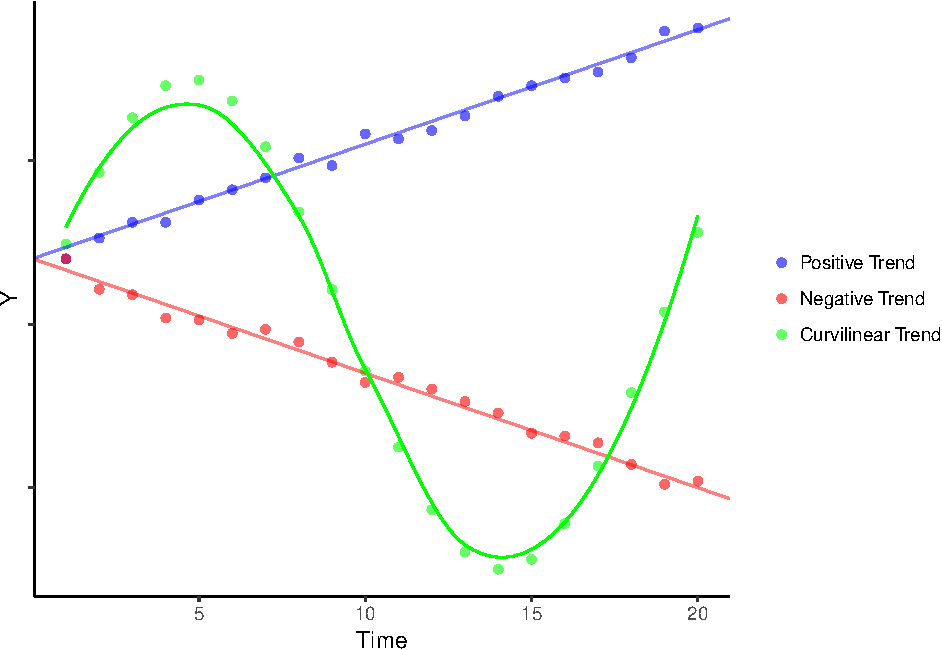
\includegraphics{figures/unnamed-chunk-12-1.pdf}
\caption{\label{fig:unnamed-chunk-12}Trend across time\label{trend}}
\end{figure}

\begin{figure}
\centering
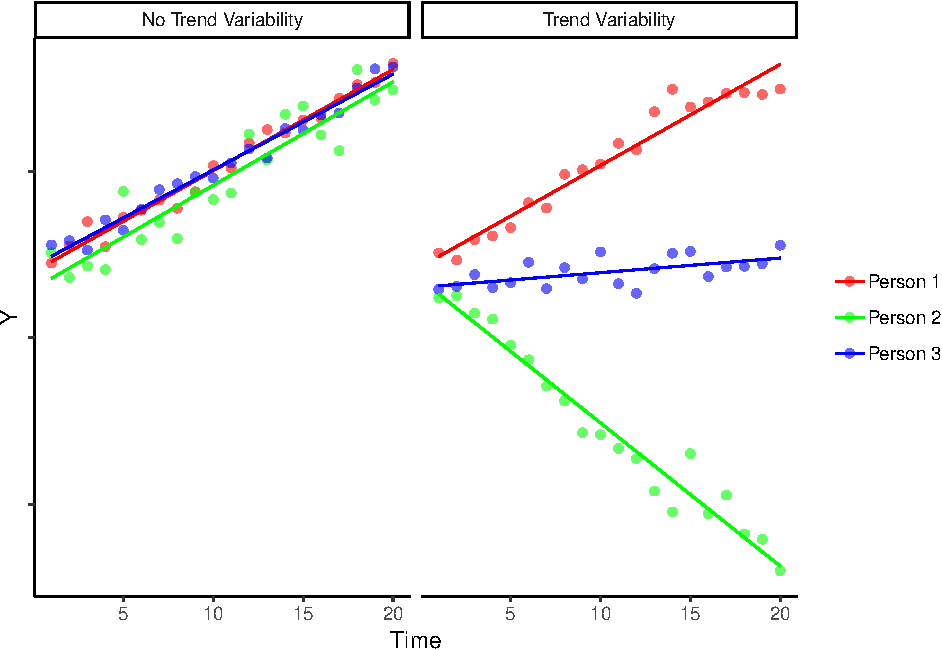
\includegraphics{figures/unnamed-chunk-13-1.pdf}
\caption{\label{fig:unnamed-chunk-13}Differences in trend variability across
units\label{trend_var}}
\end{figure}

\begin{figure}
\centering
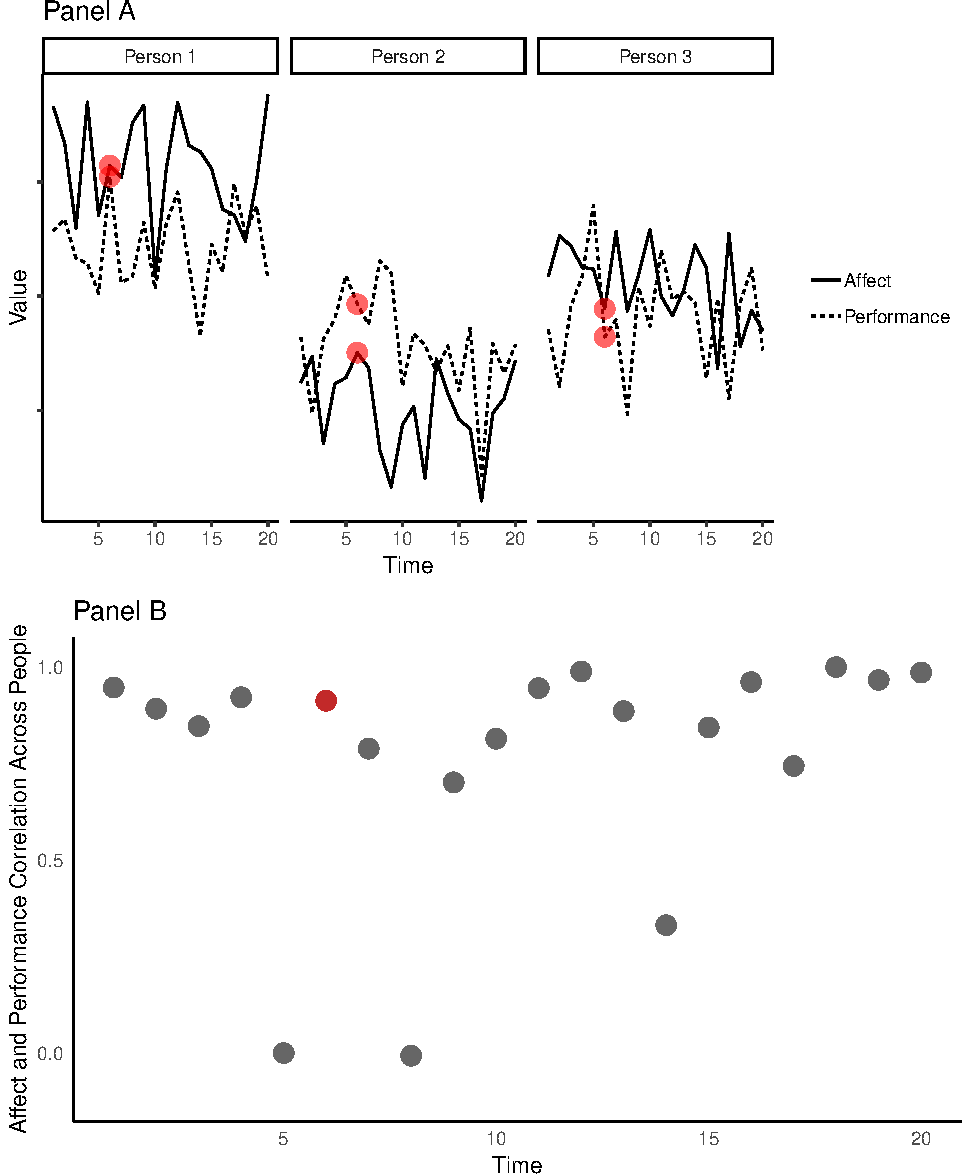
\includegraphics{figures/unnamed-chunk-14-1.pdf}
\caption{\label{fig:unnamed-chunk-14}Correlating slopes, or relating the
affect to performance trend\label{trend_correlation}}
\end{figure}

\hypertarget{models-1}{%
\subsection{Models}\label{models-1}}

Trends are called slope estimates in the statistical modeling
literature. They are also referred to as growth. Mean estimates of
slopes, or trends, or growth will tell you about trend, whereas the
variance estimates will tell you about variability across units. Growth
curves in SEM or HLM. Bivariate growth curves.

\hypertarget{dynamics}{%
\section{Dynamics}\label{dynamics}}

Dynamics refers to a specific branch of mathematics, but the term is
used in different ways throughout our literature. It is used informally
to mean \enquote{change}, \enquote{fluctuating,} \enquote{volatile,}
\enquote{longitudinal,} or \enquote{over time} (among others), whereas
formal definitions in our literature are presented within certain
contexts. Wang defines a dynamic \emph{model} as a
\enquote{representation of a system that evolves over time. In
particular it describes how the system evolves from a given state at
time \emph{t} to another state at time \emph{t + 1} as governed by the
transition rules and potential external inputs} (p.~242). Vancouver
states that dynamic \emph{variables} \enquote{behave as if they have
memory; that is, their value at any one time depends somewhat on their
previous value} (p.~604). Finally, Monge suggests that in dynamic
\emph{analyses}, \enquote{it is essential to know how variables depend
upon their own past history} (p.~409).

The crucial notion to take from dynamics, then, is memory. When the past
matters, and future states are constrained by where they were at prior
points in time, dynamics are at play. In this section, we unpack a
variety of inferences that are couched in this idea.

Does performance relate to itself over time? Do current helping
behaviors depend on prior helping behaviors? Does unit climate
demonstrate self-similarity across time? Does income now predict income
in the future? These are questions about the relationship of a single
variable with itself over time. Does it predict itself at each
subsequent moment?

Figure \ref{dynamics} (no graph yet) shows the concept graphically.
Paragraph about the graph.

The statistical term used to describe self-similarity is autoregression,
and we use it to put a label on this first inference.

\hypertarget{inference-1-there-is-autoregression-in-x.}{%
\paragraph{\texorpdfstring{Inference 1: There is autoregression in
\(x\).}{Inference 1: There is autoregression in x.}}\label{inference-1-there-is-autoregression-in-x.}}

Inference one was of course about a single variable, what about when we
apply the concept of memory to the relationship among multiple
variables? This raises the question of how one variable relates to
another at a future time. Does affect predict subsequent performance? Do
prior counterproductive work behaviors relate to current incivility?
When goal discrepancy is large (high), is effort at the subsequent time
point also high? When prior depletion is low, is current emotional
exhaustion high?

We can capture this second inference by relating current values on one
variable to future values on another. Equivalently, we can relate prior
values on one variable to current values on another. Figure
\ref{dynamics_cl} (no figure yet) plots\ldots{}Paragraph about the
graph.

Relating current to future (or prior to current) from one variable to
another is called a \enquote{cross lag} relationship.

\hypertarget{inference-2-there-is-a-cross-lag-relationship-where-one-variable-relates-to-another-at-a-different-point-in-time.-x_t-is-associated-with-y_t1-across-time.}{%
\paragraph{Inference 2: There is a cross-lag relationship, where one
variable relates to another at a different point in time. x\_t is
associated with y\_t+1 across
time.}\label{inference-2-there-is-a-cross-lag-relationship-where-one-variable-relates-to-another-at-a-different-point-in-time.-x_t-is-associated-with-y_t1-across-time.}}

Inference two tells us whether the patterns in one variable co-occur
with the patterns in another at a subsequent time point. Across time,
when affect is low is subsequent performance also low? A related
question is as follows: across time, when affect is low does performance
increase or decrease? This second question is about change. How does one
variable relate to the change in another?

When goal discrepancy is large (high), does effort increase or decrease?
When unit climate is low, do perceptions of the leader change? When
performance is high, does self efficacy go up or down?

All of these questions are about change, but an immediate question that
arises is, change from what? Baseline? The prior time point? The last
three time points? Typically change is construed with respect to the
last time point. When affect is low, does performance from the last to
the current time point increase or decrease? How does effort change from
the prior to the current time point when goal discrepancy is high?

Figure \ref{dynamics_change} demonstrates these ideas. Paragraph about
the graph.

It is typical to think of change from the prior to the current time
point, but researchers are free to move it as they please. Here are the
two final inferences that capture change in different locations.

\hypertarget{inference-3-there-is-a-change-relationship-where-one-variable-relates-to-the-change-in-another.-x_t-is-associated-with-delta-y_t.}{%
\paragraph{\texorpdfstring{Inference 3: There is a change relationship,
where one variable relates to the change in another. x\_t is associated
with \(\Delta\)
y\_t.}{Inference 3: There is a change relationship, where one variable relates to the change in another. x\_t is associated with \textbackslash{}Delta y\_t.}}\label{inference-3-there-is-a-change-relationship-where-one-variable-relates-to-the-change-in-another.-x_t-is-associated-with-delta-y_t.}}

\hypertarget{inference-4-there-is-a-cross-lag-relationship-of-change-where-one-variable-relates-to-the-change-of-another-at-a-different-point-in-time.-x_t-is-associated-with-delta-y_t1.}{%
\paragraph{\texorpdfstring{Inference 4: There is a cross-lag
relationship of change, where one variable relates to the change of
another at a different point in time. x\_t is associated with \(\Delta\)
y\_t+1.}{Inference 4: There is a cross-lag relationship of change, where one variable relates to the change of another at a different point in time. x\_t is associated with \textbackslash{}Delta y\_t+1.}}\label{inference-4-there-is-a-cross-lag-relationship-of-change-where-one-variable-relates-to-the-change-of-another-at-a-different-point-in-time.-x_t-is-associated-with-delta-y_t1.}}

\hypertarget{dynamics-inference-table}{%
\subsection{Dynamics Inference Table}\label{dynamics-inference-table}}

Again, we provide an inference table below -- this time with respect to
dynamic inferences. Inference one is about autoregression, or memory in
a single variable. Inference two asks how a variable at one time
co-occurs with another at a different time. Inferences three and four
try to understand change: when one variable is high or low, does it
relate to the change (an increase or decrease) in the values of another
variable.

\begin{tabular}{>{\raggedright\arraybackslash}p{5em}>{\raggedright\arraybackslash}p{30em}}
\toprule
Inference & Examples\\
\midrule
1 & Burnout demonstrates self-similarity across time.\newline Performance relates to subsequent performance.\\
\hline
2 & Affect predicts subsequent counterproductive work behaviors.\newline Turnover relates to subsequent firm performance.\\
\hline
3 & Positive health status relates to change in happiness.\newline Anxiety relates to change in performance.\\
\hline
4 & Affect relates to subsequent change in performance.\newline Helping behaviors predict subsequent depletion changes.\\
\bottomrule
\end{tabular}

\hypertarget{models-2}{%
\subsection{Models}\label{models-2}}

Our literature has a history with difference scores and partialling. We
debated difference scores so we have converged to partialling models.
Typical we create a model with prior values of the response variable as
a predictor.

\hypertarget{mediation}{%
\section{Mediation}\label{mediation}}

Systems of variables. Reciprocal relationships.

\hypertarget{discussion}{%
\section{Discussion}\label{discussion}}

Points to include. 1) Econometrics modeling levels vs.~modeling
differences.

\begin{enumerate}
\def\labelenumi{\arabic{enumi})}
\setcounter{enumi}{1}
\tightlist
\item
  Keep in mind you might see weird stuff in the literature. X at time 1
  relates to Z at time 2, which relates to Y at time 3, but none are
  measured repeatedly across time. This is no good. We opened with
  \enquote{we couch ourselves by only discussing studies where
  constructs were measured on each \(i\) at each \(t\).} Sometimes this
  doesn't happen\ldots{}
\end{enumerate}

\newpage

\hypertarget{references}{%
\section{References}\label{references}}

\begin{Shaded}
\begin{Highlighting}[]
\KeywordTok{r_refs}\NormalTok{(}\DataTypeTok{file =} \StringTok{"references.bib"}\NormalTok{)}
\end{Highlighting}
\end{Shaded}

\setlength{\parindent}{-0.5in}
\setlength{\leftskip}{0.5in}

\hypertarget{refs}{}
\leavevmode\hypertarget{ref-beal_esm_2015}{}%
Beal, D. J. (2015). ESM 2.0: State of the art and future potential of
experience sampling methods in organizational research. \emph{Annu. Rev.
Organ. Psychol. Organ. Behav.}, \emph{2}(1), 383--407.

\leavevmode\hypertarget{ref-hardy_interrelationships_2018}{}%
Hardy, J. H., Day, E. A., \& Steele, L. M. (2018). Interrelationships
Among Self-Regulated Learning Processes: Toward a Dynamic Process-Based
Model of Self-Regulated Learning. \emph{Journal of Management},
0149206318780440.
doi:\href{https://doi.org/10.1177/0149206318780440}{10.1177/0149206318780440}

\leavevmode\hypertarget{ref-ilgen_computational_2000}{}%
Ilgen, D. R., \& Hulin, C. L. (2000). \emph{Computational modeling of
behavior in organizations: The third scientific discipline.} American
Psychological Association.

\leavevmode\hypertarget{ref-johnson_good_2014}{}%
Johnson, R. E., Lanaj, K., \& Barnes, C. M. (2014). The good and bad of
being fair: Effects of procedural and interpersonal justice behaviors on
regulatory resources. \emph{Journal of Applied Psychology},
\emph{99}(4), 635.

\leavevmode\hypertarget{ref-jones_baby_2016}{}%
Jones, K. P., King, E. B., Gilrane, V. L., McCausland, T. C., Cortina,
J. M., \& Grimm, K. J. (2016). The baby bump: Managing a dynamic stigma
over time. \emph{Journal of Management}, \emph{42}(6), 1530--1556.

\leavevmode\hypertarget{ref-koopman_integrating_2016}{}%
Koopman, J., Lanaj, K., \& Scott, B. A. (2016). Integrating the Bright
and Dark Sides of OCB: A Daily Investigation of the Benefits and Costs
of Helping Others. \emph{Academy of Management Journal}, \emph{59}(2),
414--435.
doi:\href{https://doi.org/10.5465/amj.2014.0262}{10.5465/amj.2014.0262}

\leavevmode\hypertarget{ref-kozlowski_work_2003}{}%
Kozlowski, S. W., \& Bell, B. S. (2003). Work groups and teams in
organizations. \emph{Handbook of Psychology}, 333--375.

\leavevmode\hypertarget{ref-meier_reciprocal_2013}{}%
Meier, L. L., \& Spector, P. E. (2013). Reciprocal effects of work
stressors and counterproductive work behavior: A five-wave longitudinal
study. \emph{Journal of Applied Psychology}, \emph{98}(3), 529.

\leavevmode\hypertarget{ref-pitariu_explaining_2010}{}%
Pitariu, A. H., \& Ployhart, R. E. (2010). Explaining change: Theorizing
and testing dynamic mediated longitudinal relationships. \emph{Journal
of Management}, \emph{36}(2), 405--429.

\leavevmode\hypertarget{ref-ployhart_longitudinal_2010}{}%
Ployhart, R. E., \& Vandenberg, R. J. (2010). Longitudinal research: The
theory, design, and analysis of change. \emph{Journal of Management},
\emph{36}(1), 94--120.

\leavevmode\hypertarget{ref-ritter_understanding_2016}{}%
Ritter, K.-J., Matthews, R. A., Ford, M. T., \& Henderson, A. A. (2016).
Understanding role stressors and job satisfaction over time using
adaptation theory. \emph{Journal of Applied Psychology}, \emph{101}(12),
1655.

\leavevmode\hypertarget{ref-rosen_who_2016}{}%
Rosen, C. C., Koopman, J., Gabriel, A. S., \& Johnson, R. E. (2016). Who
strikes back? A daily investigation of when and why incivility begets
incivility. \emph{Journal of Applied Psychology}, \emph{101}(11), 1620.


\end{document}
